\documentclass[polish,a4paper]{article}
\usepackage{amsmath}
\usepackage{amssymb, amsfonts, amsthm, amsmath, bm}
\usepackage[T1]{fontenc}
\usepackage[utf8]{inputenc}
\usepackage{babel}
\usepackage{pslatex}
\usepackage{pgfplots}
\usepackage{hhline}
\usepackage[american]{circuitikz} 
\usepackage{anysize}
\usepackage{graphicx}
\DeclareGraphicsExtensions{.jpg}
\marginsize{2.5cm}{2.5cm}{3cm}{3cm}
\bibliographystyle{IEEEtran}


%makro do indeksów w tabeli
\newcommand{\PRzFieldDsc}[1]{\sffamily\bfseries\scriptsize #1}

%makro do informacji w tabeli
\newcommand{\PRzFieldCnt}[1]{\itshape #1}

%potężne makro tworzące tabelę z informacjami o teamie
\newcommand{\PRzHeading}[8]{
%% #1 - nazwa laboratorium
%% #2 - kierunek 
%% #3 - specjalność 
%% #4 - rok studiów 
%% #5 - symbol grupy lab.
%% #6 - temat 
%% #7 - numer lab.
%% #8 - skład grupy ćwiczeniowej

\begin{center}
\begin{tabular}{ p{0.32\textwidth} p{0.15\textwidth} p{0.15\textwidth} p{0.12\textwidth} p{0.12\textwidth} }

  &   &   &   &   \\
\hline
\multicolumn{5}{|c|}{}\\[-1ex]
\multicolumn{5}{|c|}{{\LARGE #1}}\\
\multicolumn{5}{|c|}{}\\[-1ex]

\hline
\multicolumn{1}{|l|}{\PRzFieldDsc{Kierunek}}	& \multicolumn{1}{|l|}{\PRzFieldDsc{Specjalność}}	& \multicolumn{1}{|l|}{\PRzFieldDsc{Rok studiów}}	& \multicolumn{2}{|l|}{\PRzFieldDsc{Symbol grupy lab.}} \\
\multicolumn{1}{|c|}{\PRzFieldCnt{#2}}		& \multicolumn{1}{|c|}{\PRzFieldCnt{#3}}		& \multicolumn{1}{|c|}{\PRzFieldCnt{#4}}		& \multicolumn{2}{|c|}{\PRzFieldCnt{#5}} \\

\hline
\multicolumn{4}{|l|}{\PRzFieldDsc{Temat Laboratorium}}		& \multicolumn{1}{|l|}{\PRzFieldDsc{Numer lab.}} \\
\multicolumn{4}{|c|}{\PRzFieldCnt{#6}}				& \multicolumn{1}{|c|}{\PRzFieldCnt{#7}} \\

\hline
\multicolumn{5}{|l|}{\PRzFieldDsc{Skład grupy ćwiczeniowej oraz numery indeksów}}\\
\multicolumn{5}{|c|}{\PRzFieldCnt{#8}}\\

\hline
\multicolumn{3}{|l|}{\PRzFieldDsc{Uwagi}}	& \multicolumn{2}{|l|}{\PRzFieldDsc{Ocena}} \\
\multicolumn{3}{|c|}{\PRzFieldCnt{\ }}		& \multicolumn{2}{|c|}{\PRzFieldCnt{\ }} \\

\hline
\end{tabular}
\end{center}
}
%koniec potężnego makro do tabeli

\begin{document}

%stworzenie tabeli - miejsce na zmienianie danych w tabeli
%indeksy do uzupełnienia
\PRzHeading{Laboratorium Podstaw Elektroniki}{Informatyka}{--}{I}{I1}{Tranzystory}{5}{Ewa Fengler(132219), Sebastian Maciejewski(132275), Jan Techner(132332)}{}

%ZADANIA

\section*{Cel}
Celem przeprowadzanych ćwiczeń jest zapoznanie się z właściwościami tranzystora MOSFET jako elementu elektronicznego w układach prądu stałego oraz zmiennego.

\section{Zadanie 1.5}
Badanie zależności pomiędzy sygnałem sterującym a sterowanym dla tranzystora nMOS.

\subsection*{1.}
\begin{figure}[!h]
\centering
\begin{circuitikz}[scale=1, font = \scriptsize, european voltages]
\draw (0,0) to [american current source, o-o, l=$5V$] (0,2) -- (0,4) to [esource] (3,4) to [R, l=$R_1$, a=1k$\Omega$, i^>=$I_D$] (6,4)-- (6,3)
(6,1.5) -- (6,0)-- (0,0)
(2,0) to [american current source, o-o, l=$0..5V$] (2,2)
(3.5, 0) to [esource, *-*] (3.5,2)
(2,2) -- (5.1,2)
(4.5, 0.3) -- (4.5,1.4) ;


\draw (6,2.27) node[nigfete,bodydiode](pnp){}
(2,-0.05) node [rground] {}
(2, -0.6) node {GND}
(6.2, 3) node {D}
(6.2, 1.5) node {S}
(5.1, 2.2) node {G}
(6.4, 2.17) node [right, scale = 0.8] {Q1}
(6.4, 2.37) node [right, scale = 0.8] {BS170}

(1.5, 4) node {mA}
(3.5, 1) node {V}
(4.5, 1.4) node [vcc, scale = 0.7]{}
(4.8, 1) node {$U_{GS}$}
;

\end{circuitikz}
\caption{Obw. 1.6 Układ do badania charakterystyki bramkowej tranzystora nMOS}
\label{fig:obw1.6}
\end{figure}



\subsection*{2.}
Pomiary prądu drenu $I_D$ w zależności od napięcia bramka - źródło $U_{GS}$ z uwzględnieniem szczególnej wartości $U_{GS}$, przy której gwałtownie wzrasta natężenie prądu - $1,9V$.

\begin{center}
\begin{tabular}{|l|l|}
\hline
\textbf{$U_{GS} [V]$} & \textbf{$I_D [mA]$}\\
\hhline{|=|=|}

0 & 0\\
\hline
0,5 & 0\\
\hline
1 & 0\\
\hline
1,9 & 0,16\\
\hline
2 & 0,57\\
\hline
2,1 & 2,07\\
\hline
2,2 & 3,17\\
\hline
2,3 & 4,95\\
\hline
2,4 & 5,02\\
\hline
2,5 & 5,03\\
\hline
3 & 5,05\\
\hline
3,5 & 5,05\\
\hline
4 & 5,05\\
\hline
4,5 & 5,06\\
\hline
5 & 5,06\\
\hline

\end{tabular}
\end{center}


\subsection*{3.}
% Na podstawie zarejestrowanych wartości utwórz wykres w sprawozdaniu z wykonania ćwiczenia.
%4.  Odczytaj z noty katalogowej producenta tranzystora wartość napięcia progowego Uth. Nanieś odczytaną wartość na wykres.

\begin{figure}[!h]
\centering
\begin{tikzpicture}[scale=1]
\begin{axis}[
xlabel={Napięcie Bramka-Źródło [V]},
ylabel={Prąd drenu [mA]},
xmin=0,xmax=5.5,
ymin=0,ymax=7,
legend pos=north east,
ymajorgrids=true,grid style=dashed
]

\addplot[smooth, tension={0.3}, red, mark=*, mark size = {1pt}]
coordinates {
(0,0)
(0.5,0)
(1,0)
(1.9,0.16)
(2,0.57)
(2.1,2.07)
(2.2,3.17)
(2.3,4.95)
(2.4,5.02)
(2.5, 5.03)
(3,5.05)
(3.5,5.05)
(4,5.05)
(4.5,5.06)
(5, 5.06)
};

\addplot[cyan, line width = 0.6mm]
coordinates {
(0.8,0)
(0.8,5.1)
};

\addplot[dashed, cyan, line width = 0.6mm]
coordinates {
(2,0)
(2,5.1)
};

\addplot[cyan, line width = 0.6mm]
coordinates {
(3,0)
(3,5.1)
};

\legend{wykres zależności,wartości graniczne}
\end{axis}
\end{tikzpicture}
\caption{Wartości prądu drenu $I_D$ w zależności od napięcia Bramka Źródło $U_{GS}$ dla tranzystora nMOS}
\label{fig:wykres1}
\end{figure}

\subsection*{4.}
Minimalna wartość napięcia progowego odczytana z noty katalogowej producenta wynosi $0,8V$, typowa wartość to $2,0V$, zaś wartość maksymalna wynosi $3,0V$.

\subsection*{5.}

Wyniki pomiarów wskazują, że badany tranzystor zaczyna przewodzić gdy napięcie bramka-źródło przekroczy wartość $1,9V$. Jest to zgodne z danymi katalogowymi tranzystora, które napięcie progowe (napięcie odcięcia) określają jako większe od $0,8V$, a mniejsze od $3,0V$, typowo $2,0V$. Oznacza to, że zmierzona wartość napięcia progowego jest tylko nieznacznie mniejsza od wartości typowej. 


\section{Zadanie 1.6}

Badanie działania tranzystora pMOS.

\subsection*{1.}

\begin{figure}[!h]
\centering
\begin{circuitikz}[scale=1, font = \scriptsize, european voltages]
\draw (0,0) to [american current source, o-o, l=$5V$] (0,2) -- (0,4) -- (6,4)-- (6,3)
(6, 2.1) to [R, l_=$R_7$, a^=1k$\Omega$, i>_=$I_D$] (6,0) to [esource] (3.5,0) -- (0,0)
(2,0) to [american current source, o-, l=$0..5V$] (2,2) to [short, -o] (2, 3.07)
(3.5, 0) to [esource, *-] (3.5,2) to [short, -*] (3.5,3.07)
(2,3.07) -- (5.1,3.07)
(4.1, 0.3) -- (4.1,2.5)
(-1.3, 0.3) -- (-1.3,3.5)
(4.6, 3.8) -- (4.6,3.5) ;


\draw (6,2.8) node[pigfete,bodydiode](pnp){}
(2,-0.05) node [rground] {}
(2, -0.6) node {GND}
(6.2, 3.48) node {S}
(6.2, 2.08) node {D}
(5.1, 3.3) node {G}
(6.4, 2.7) node [right, scale = 0.8] {Q4}
(6.4, 2.9) node [right, scale = 0.8] {BS250}

(4.75, 0) node {mA}
(3.5, 1) node {V}
(4.1, 2.5) node [vcc, scale = 0.7]{}
(-1.3, 3.4) node [vcc, scale = 0.7]{}
(4.6, 3.6) node [vcc, scale = 0.7, rotate = 180]{}
(4.3, 1.4) node {$U_1$}
(-1.6, 2) node {$U_{SS}$}
(4.3, 3.55) node {$U_{GS}$}
;

\end{circuitikz}
\caption{Obw. 1.7 Układ do badania charakterystyki bramkowej tranzystora pMOS}
\label{fig:obw1.7}
\end{figure}

\subsection*{2.}

Pomiary prądu drenu $I_D$ w zależności od napięcia źródła $U_{1}$ z uwzględnieniem szczególnej wartości $U_{1}$, przy której gwałtownie wzrasta natężenie prądu. Dla wszystkich pomiarów obliczone zostało także napięcie bramka - źródło $U_{GS}$ na podstawie napięciowego prawa Kirchhoffa, ze wzoru $U_{GS}=-(U_{SS}-U_1)$.\\
Widać dla jakiej wartości $V1$ prąd drenu zaczyna gwałtownie spadać - jest to napięcie skojarzone z progiem załączenia tranzystora: $2V$, to oznacza, że napięcie bramka-źródło wynosiło $-3V$ - ta wartość mieści się w przedziale z noty katalogowej.

\begin{center}
\begin{tabular}{|l|l|l|}
\hline
\textbf{$U_1 [V]$} & \textbf{$I_D [mA]$} & \textbf{$U_{GS} [V]$}\\
\hhline{|=|=|=|}
0 & 5,04 & -5\\
\hline
0,5 & 5,03 & -4,5\\
\hline
1 & 5,01 & -4\\
\hline
1,5 & 4,9 & -3,5\\
\hline
1,6 & 2,09 & -3,4\\
\hline
1,7 & 1,36 & -3,3\\
\hline
1,8 & 0,57 & -3,2\\
\hline
1,9 & 0,27 & -3,1\\
\hline
2 & 0,08 & -3\\
\hline
2,5 & 0 & -2,5\\
\hline
3 & 0 & -2\\
\hline
3,5 & 0 & -1,5\\
\hline
4 & 0 & -1\\
\hline
4,5 & 0 & -0,5\\
\hline
5 & 0 & 0\\
\hline

\end{tabular}
\end{center}


\subsection*{3.} 

\begin{figure}[!h]
\centering
\begin{tikzpicture}[scale=1]
\begin{axis}[
xlabel={Napięcie Bramka-Źródło [V]},
ylabel={Prąd drenu [mA]},
xmin=-5.5,xmax = 0,
ymin=0,ymax=7,
legend pos=north east,
ymajorgrids=true,grid style=dashed
]

\addplot[smooth, tension={0.3}, red, mark=*, mark size = {1pt}]
coordinates {
(-5,5.04)
(-4.5,5.03)
(-4,5.01)
(-3.5,4.9)
(-3.4,2.09)
(-3.3,1.36)
(-3.2,0.57)
(-3.1,0.27)
(-3,0.08)
(-2.5,0)
(-2,0)
(-1.5,0)
(-1,0)
(-0.5,0)
(0, 0)
};

\addplot[cyan, line width = 0.6mm]
coordinates {
(-1,0)
(-1,5.1)
};

\addplot[dashed, cyan, line width = 0.6mm]
coordinates {
(2,0)
(2,5.1)
};

\addplot[cyan, line width = 0.6mm]
coordinates {
(-3.5,0)
(-3.5,5.1)
};

\legend{wykres zależności,wartości graniczne}
\end{axis}
\end{tikzpicture}
\caption{Wartości prądu drenu $I_D$ w zależności od napięcia Bramka Źródło $U_{GS}$ dla tranzystora pMOS}
\label{fig:wykres2}
\end{figure}
% Na podstawie zarejestrowanych wartości utwórz wykres Wartości prądu drenu w funkcji napięcia Bramka- Źródło U_GS. Zwróć uwagę, że bieżącym sposobie włączenia tranzystora do obwodu, wartości U_GS będą ujemne.
% 4. Odczytaj z noty katalogowej producenta tranzystora wartość napięcia progowego Uth. Nanieś odczytaną wartość na wykres.


\subsection*{4.}
Dla używanego tranzystora progowe wartości napięcia odczytane z noty katalogowej producenta wynoszą minimum $-1V$ i maksimum $-3,5V$.\\
Wyniki pomiarów wskazują, że badany tranzystor zaczyna przewodzić gdy napięcie bramka-źródło przekroczy $-3V$. Zmierzona wartość należy do zakresu określonego przez dane katalogowe tranzystora, które napięcie progowe (napięcie odcięcia) określają jako wartość z przedziału  od $-1V$ do $-3,5V$, zatem parametry danego tranzystora zgadzają się z danymi katalogowymi.


\section{Zadanie 1.7}

Badanie charakterystyki drenowej tranzystora nMOS.

\subsection*{1.}

\begin{figure}[!h]
\centering
\begin{circuitikz}[scale=1, font = \scriptsize, european voltages]
\draw (0,0) to [american current source, o-o, l=$0..10V$] (0,2) -- (0,4) to [esource] (2.5,4) to [R, l=$R_2$, a=1k$\Omega$, i^>=$I_D$, -*] (5,4)-- (5,3)
(5,1.5) -- (5,0) to [short, *-] (0,0)
(2,0) to [american current source, o-o, l=$5V$] (2,2)
(2,2) -- (4.1,2)

(5.6, 1.1) -- (5.6,3.2) 
(5, 0) -- (6.5,0) to [esource] (6.5,4) -- (5,4)
;

\draw (5,2.27) node[nigfete,bodydiode](pnp){}
(5.2, 3) node {D}
(5.2, 1.5) node {S}
(4.1, 2.2) node {G}
(4.9, 2.9) node [left, scale = 0.8] {Q2}
(4.9, 3.1) node [left, scale = 0.8] {BS170}
(1.25, 4) node {mA}
(6.5, 2) node {V}
(5.6, 3.2) node [vcc, scale = 0.7]{}
(5.9, 2.5) node {$U_{DS}$}
;

\end{circuitikz}
\caption{Obw. 1.8 Układ do badania charakterystyki drenowej tranzystora nMOS}
\label{fig:obw1.8}
\end{figure}

\subsection*{2.}
Napięcie bramka-źródło $U_{GS} = 5,05V$

%napięcie dren - źródło | I_D

\begin{center}
\begin{tabular}{|l|l|}
\hline
\textbf{$U_{DS} [mV]$} & \textbf{$I_d [mA]$}\\
\hhline{|=|=|}

0 & 0\\
\hline
3,2 & 1,16 \\
\hline
6,1 & 2,23 \\
\hline
8,7 & 3,14 \\
\hline
11,3 & 4,15 \\
\hline
14,0 & 5,18 \\
\hline
16,7 & 6,19 \\
\hline
19,4 & 7,19 \\
\hline
22,2 & 8,19 \\
\hline
25 & 9,24 \\
\hline
27,9 & 10,29 \\
\hline

\end{tabular}
\end{center}

\subsection*{3.}

\begin{figure}[!h]
\centering
\begin{circuitikz}[scale=1, font = \scriptsize, european voltages]
\draw (0,0) to [american current source, o-o, l=$0..10V$] (0,2) -- (0,4) to [esource] (2.5,4) to [R, l=$R_3$, a=1k$\Omega$, i^>=$I_D$, -*] (5,4)-- (5,3)
(5,1.5) -- (5,0) to [short, *-] (0,0)
(1.5,0) to [american current source, o-o] (1.5,2)
(1.5,2) to [R, l=$R_4$, a=1k$\Omega$, -*] (3.7,2) -- (4.1, 2)
(3.7, 0) to [R, l=$R_5$, a=1k$\Omega$, *-] (3.7,2)
(5.6, 1.1) -- (5.6,3.2) 
(5, 0) -- (6.5,0) to [esource] (6.5,4) -- (5,4)
;

\draw (5,2.27) node[nigfete,bodydiode](pnp){}
(5.2, 3) node {D}
(5.2, 1.5) node {S}
(4.1, 2.2) node {G}
(4.9, 2.9) node [left, scale = 0.8] {Q3}
(4.9, 3.1) node [left, scale = 0.8] {BS170}
(1.25, 4) node {mA}
(6.5, 2) node {V}
(1.2, 1.6) node {$5V$}
(5.6, 3.2) node [vcc, scale = 0.7]{}
(5.9, 2.5) node {$U_{DS}$}
;

\end{circuitikz}
\caption{Obw. 1.9 Układ do badania charakterystyki drenowej dla obniżonego napięcia bramki}
\label{fig:obw1.9}
\end{figure}

\subsection*{4.}

Napięcie bramka-źródło $U_{GS} = 2,52V$

\begin{center}
\begin{tabular}{|l|l|}
\hline
\textbf{$U_{DS} [mV]$} & \textbf{$I_D [mA]$}\\
\hhline{|=|=|}
0 & 0 \\
\hline
12,7 & 1,17 \\
\hline
24 & 2,12 \\
\hline
37,6 & 3,16 \\
\hline
52,3 & 4,14 \\
\hline
68,8 & 5,10 \\
\hline
89,6 & 6,10 \\
\hline
116,3 & 7,12 \\
\hline
150,1 & 8,06 \\
\hline
205 & 9,09 \\
\hline
298& 9,94 \\
\hline

\end{tabular}
\end{center}
\begin{figure}[!h]
\centering
\begin{tikzpicture}[scale=1]
\begin{axis}[
xlabel={Napięcie Dren-Źródło [mV]},
ylabel={Prąd drenu [mA]},
xmin=0,xmax=330,
ymin=0,ymax=12,
legend pos=south east,
ymajorgrids=true,grid style=dashed
]

\addplot[smooth, tension={0.3}, green, mark=*, mark size = {1pt}]
coordinates {
(0,0)
(12.7,1.17)
(24,2.12)
(37.6,3.16)
(52.3,4.14)
(68.8,5.10)
(89.6,6.10)
(116.3,7.12)
(150.1,8.06)
(205, 9.09)
(298,9.94)
};

\legend{$U_{GS} = 2.52V$}
\end{axis}
\end{tikzpicture}
\caption{Wartości prądu drenu $I_D$ w zależności od napięcia Dren-Źródło $U_{DS}$ dla tranzystora nMOS przy obniżonym napięciu bramki}
\label{fig:wykres4}
\end{figure}

\subsection*{5.}
% Wartości pomiarów uzyskanych w obwodach z rys 1.8 oraz 1.9 zobrazuj na wspólnym wykresie. Przy obydwu krzywych napisz wartości napięć bramki U_GS jakie występowało w trakcie badania.
\begin{figure}[!h]
\centering
\begin{tikzpicture}[scale=1]
\begin{axis}[
xlabel={Napięcie Dren-Źródło [mV]},
ylabel={Prąd drenu [mA]},
xmin=0,xmax=330,
ymin=0,ymax=12,
legend pos=south east,
ymajorgrids=true,grid style=dashed
]

\addplot[smooth, tension={0.3}, red, mark=*, mark size = {1pt}]
coordinates {
(0,0)
(3.2,1.16)
(6.1,2.23)
(8.7,3.14)
(11.3,4.15)
(14,5.18)
(16.7,6.19)
(19.4,7.19)
(22.2,8.19)
(25, 9.24)
(27.9,10.29)
};

\addplot[smooth, tension={0.3}, green, mark=*, mark size = {1pt}]
coordinates {
(0,0)
(12.7,1.17)
(24,2.12)
(37.6,3.16)
(52.3,4.14)
(68.8,5.10)
(89.6,6.10)
(116.3,7.12)
(150.1,8.06)
(205, 9.09)
(298,9.94)
};

\legend{$U_{GS} = 5.05V$,$U_{GS} = 2.52V$}
\end{axis}
\end{tikzpicture}
\caption{Wartości prądu drenu $I_D$ w zależności od napięcia Dren-Źródło $U_{DS}$ dla tranzystora nMOS dla różnych napięć bramki}
\label{fig:wykres3}
\end{figure}

\subsection*{6.}
Wykonane pomiary obejmowały fragment charakterystyki drenowej (wyjściowej) tranzystora MOS dla niewielkich napięć dren-źródło. Na wykresie zielonym możemy obserwować zarówno fragment charakterystyki w obszarze liniowym jak i początkowym obszarze nasycenia. Jest to możliwe dzięki temu, że napięcie bramka-źródło ($2,52V$) jest bliskie napięciu odcięcia wcześniej zmierzonego. Charakterystyka czerwona obejmuje wyłącznie fragment liniowej charakterystyki wyjściowej, ponieważ wysoka wartość rezystancji umieszczonej w drenie tranzystora $(1k\Omega)$, oraz niezbyt wysoka wartość napięcia zasilającego ($10V$) nie pozwoliła na badanie charakterystyki dla prądów drenu większych niż $10mA$. Stąd wniosek, że prąd nasycenia drenu dla napięcia Bramka-Źródło równego $5,05V$ musi być wielokrotnie większy od $10mA$.


\newpage
\section{Zadanie 1.8}

Badanie charakterystyki drenowej tranzystora pMOS.

\subsection*{1.}

\begin{figure}[!h]
\centering
\begin{circuitikz}[scale=1, font = \scriptsize, european voltages]
\draw (0,0) to [american current source, o-o] (0,2) -- (0,4) -- (5,4)-- (5,3)
(5, 2.1) to [R, l_=$R_6$, a^=1k$\Omega$, i>_=$I_D$] (5,0) to [esource] (2,0) -- (0,0)
(2,0) to [american current source, o-] (2,2) to [short, -o] (2, 3.07)
(2, 3.07) -- (4.1,3.07)

(-1.3, 0.3) -- (-1.3,3.5)

(5, 0) -- (6.5,0) to [esource] (6.5,4) -- (5,4)
 ;


\draw (5,2.8) node[pigfete,bodydiode](pnp){}
(2,-0.05) node [rground] {}
(5.2, 3.48) node {S}
(5.2, 2.08) node {D}
(4.1, 3.3) node {G}
(5.4, 2.7) node [right, scale = 0.8] {Q5}
(5.4, 2.9) node [right, scale = 0.8] {BS250}
(2, -0.6) node {GND}
(3.5, 0) node {mA}
(6.5, 2) node {V}
(-1.3, 3.4) node [vcc, scale = 0.7]{}
(-1.6, 2) node {$U_{SD}$}
(1.7, 1.6) node {$5V$}
(-0.5, 1.6) node {$0..10V$}
;

\end{circuitikz}
\caption{Obw. 1.10 Układ do badania charakterystyki drenowej tranzystora pMOS
}
\label{fig:obw1.10}
\end{figure}

\subsection*{2.}
Zmierzone napięcie bramki $U_{GS}$ wynosiło $-5,05V$.

%napięcie Dren - Źródło | prąd drenu
%TODO: czy te minusy w tabeli? I czy pierwsza kolumna?

\begin{center}
\begin{tabular}{|c|c|c|}
\hline
\textbf{Napięcie źródła [V]} & \textbf{$U_{DS} [V]$} & \textbf{$I_D [mA]$}\\
\hhline{|=|=|=|}

1 & -1,12 & 0 \\
\hline
2 & -2,15 & 0 \\
\hline
3 & -3,15 & 0 \\
\hline
4 & -4,24 & 0 \\
\hline
5 & -5,25 & 0 \\
\hline
6 & -6,16 & 0 \\
\hline
7 & -6,92 & 0,22 \\
\hline
7,5 & -1,46 & 6,15 \\
\hline
8 & -0,1 & 8,13 \\
\hline
9 & -0,07 & 9,20 \\
10 & -0,07 & 10,18 \\
\hline

\end{tabular}
\end{center}

\newpage
\subsection*{3.}

\begin{figure}[!h]
\centering
\begin{circuitikz}[scale=1, font = \scriptsize, european voltages]
\draw (0,0) to [american current source, o-o] (0,2) -- (0,4) -- (5,4)-- (5,3)
(5, 2.1) to [R, l_=$R_8$, a^=1k$\Omega$, i>_=$I_D$] (5,0) to [esource] (3.5,0) -- (0,0)
(1.5,0) to [american current source, o-] (1.5,2) to [short, -o] (1.5, 3.07)
(3.5, 0) to [R, l_=$R_{10}$, a^=1k$\Omega$, *-] (3.5,2) to [short, -*] (3.5,3.07)
(1.5,3.07) to [R, l=$R_9$, a=1k$\Omega$, o-] (3.5, 3.07) -- (4.1,3.07)

(-1.3, 0.3) -- (-1.3,3.5)

(5, 0) -- (6.5,0) to [esource] (6.5,4) -- (5,4)
 ;


\draw (5,2.8) node[pigfete,bodydiode](pnp){}
(1.5,-0.05) node [rground] {}
(5.2, 3.48) node {S}
(5.2, 2.08) node {D}
(4.1, 3.3) node {G}
(5.4, 2.7) node [right, scale = 0.8] {Q6}
(5.4, 2.9) node [right, scale = 0.8] {BS250}
(1.5, -0.6) node {GND}
(4.25, 0) node {mA}
(6.5, 2) node {V}
(-1.3, 3.4) node [vcc, scale = 0.7]{}
(-1.6, 2) node {$U_{SD}$}
(1.2, 1.6) node {$5V$}
(-0.5, 1.6) node {$0..10V$}
;

\end{circuitikz}
\caption{Obw. 1.11 Układ do badania charakterystyki drenowej dla obniżonego napięcia bramki pMOS}
\label{fig:obw1.11}
\end{figure}


\subsection*{4.}
Napięcie bramki $U_{GS}$ wynosiło $2,5V$.


\begin{center}
\begin{tabular}{|c|c|c|}
\hline
\textbf{Napięcie źródła [V]} & \textbf{$U_{DS} [V]$} & \textbf{$I_D [mA]$}\\
\hhline{|=|=|=|}
1 & -1,13 & 0 \\
\hline
2 & -2,18 & 0 \\
\hline
3 & -3,18 & 0 \\
\hline
4 & -4,16 & 0 \\
\hline
4,5 & -4,35 & 0,3 \\
\hline
5 & -0,27 & 4,95 \\
\hline
6 & -0,05 & 6,14 \\
\hline
7 & -0,05 & 7,19 \\
\hline
8 & -0,05 & 8,17 \\
\hline
9 & -0,06 & 9,2 \\
\hline
10 & -0,06 & 10,21 \\
\hline


\end{tabular}
\end{center}
\newpage

\subsection*{5.}
% Wartości pomiarów uzyskanych w obwodach z rys 1.10 oraz 1.11 zobrazuj na wspólnym wykresie w sprawozdaniu. Przy obydwu krzywych napisz wartości napięć bramki UGS jakie występowało w trakcie badania.
\begin{figure}[!h]
\centering
\begin{tikzpicture}[scale=1]
\begin{axis}[
xlabel={Napięcie Dren-Źródło [mV]},
ylabel={Prąd drenu [mA]},
xmin=-10,xmax=1,
ymin=0,ymax=12,
legend pos=north west,
ymajorgrids=true,grid style=dashed
]

\addplot[smooth, tension={0.3}, red, mark=*, mark size = {1pt}]
coordinates {
(-1.12,0)
(-2.15,0)
(-3.15,0)
(-4.24,0)
(-5.15,0)
(-6.16,0)
(-6.92,0.22)
(-1.46,6.15)
(-0.1,8.13)
(-0.07, 9.20)
(-0.07,10.18)
};

\addplot[smooth, tension={0.3}, green, mark=*, mark size = {1pt}]
coordinates {
(-1.13,0)
(-2.18,0)
(-3.18,0)
(-4.16,0)
(-4.35,0.3)
(-0.27,4.95)
(-0.05,6.14)
(-0.05,7.19)
(-0.05,8.17)
(-0.05, 9.2)
(-0.05,10.21)
};

\legend{$U_{GS} = -5.05V$,$U_{GS} = ?$}
\end{axis}
\end{tikzpicture}
\caption{Wartości prądu drenu $I_D$ w zależności od napięcia Dren-Źródło $U_{DS}$ dla tranzystora pMOS dla różnych napięć bramki}
\label{fig:wykres5}
\end{figure}



\subsection*{6.}
Otrzymane charakterystyki w zadaniu 1.8 są niepoprawne (nie są charakterystykami wyjściowymi lub charakterystykami drenowymi tranzystora MOS z kanałem typu p). Wynika to z błędnego układu pomiarowego, w którym:\\
1) nie było mierzone napięcie Dren-Źródło, tylko napięcie zasilające układ\\
2) napięcie Bramka-Źródło zmieniało się w trakcie każdego pomiaru po zmianie napięcia zasilającego (zależało od napięcia zasilającego)\\
Dla układu 1.10 napięcie Bramka-Źródło było równe różnicy $5V$ i napięcia zasilającego, czyli dla napięcia zasilającego $10V$ wynosiło $-5V$, a dla $1V$ wynosiło $+4V$, co spowodowało, że nie był spełniony podstawowy warunek $U_{GS} = const$ dla każdego wykresu z rodziny. Analogicznie dla schematu z rysunku 1.11: napięcie pomiędzy Bramką a Źródłem było równe $2,5V$ - napięcie zasilania.

\newpage
\section{Zadanie 1.9}

Badanie zachowania tranzystora nMOS jako przełącznika, w którym przepływem prądu można sterować przy pomocy napięcia.

\subsection*{1.}

\begin{figure}[!h]
\centering
\begin{circuitikz}[scale=1, font = \scriptsize, european voltages]
\draw (0.6, 0) -- (0,0) to  [R, l_=$R_{12}$, a^=1M$\Omega$, *-] (0,-2) to [short, -*] (1.5,-2) -- (5.5,-2) to [american current source, o-o, l^=$10V$] (5.5,0) -- (5.5, 2) -- (-1, 2) to [short, -*] (-1, 1) (0,0) to [short, -*] (-1,0)
(1.5, -2) -- (1.5, -0.5)
(5.5, 1.05) to [R, l_=$R_{11}$, a^=1k$\Omega$, *-] (3.5, 1.05) to [stroke led, l=$LED_1$, mirror] (2, 1.05) -- (1.5, 1.05)
(1.5, 1.05) -- (2, 1.05) 
;

\draw (1.5,0.27) node[nigfete,bodydiode](pnp){}
(1.4, 1.1) node [left, scale = 0.8] {Q7}
(1.4, 0.9) node [left, scale = 0.8] {BS170}
(-1, 0.5) node [scale = 1.2] {A-A}
;

\end{circuitikz}
\caption{Obw. 1.14 Schemat układu do badania tranzystora nMOS w roli przełącznika}
\label{fig:obw1.14}
\end{figure}


\subsection*{3.}
Po zwarciu palcem zacisków oznaczonych jako A - A dioda zaczęła świecić, co widać na poniższym zdjęciu:


\begin{center}
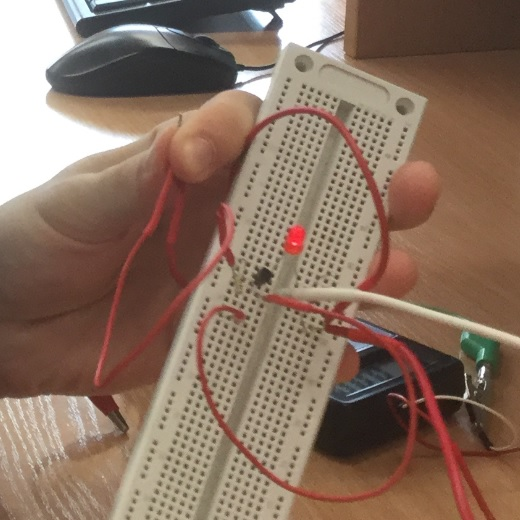
\includegraphics[scale=0.6]{zwarcie}
\end{center}


\newpage

\subsection*{4.}

\begin{figure}[!h]
\centering
\begin{circuitikz}[scale=1, font = \scriptsize, european voltages]
\draw (0.6, 0) -- (0,0) to  [R, l_=$R_{14}$, a^=47k$\Omega$, *-] (0,-2) to [short, -*] (1.5,-2) -- (5.5,-2) to [american current source, o-o, l^=$10V$] (5.5,0) -- (5.5, 2) -- (-3, 2) to [short, -*] (-3, 1) (0,0) to [short, -*] (-3,0)
(1.5, -2) -- (1.5, -0.5)
(5.5, 1.05) to [R, l_=$R_{13}$, a^=1k$\Omega$, *-] (3.5, 1.05) to [stroke led, l=$LED_2$, mirror] (2, 1.05) -- (1.5, 1.05)
(1.5, 1.05) -- (2, 1.05) 
(-2, 0) to [ecapacitor, l=$C_1$, a=100$\mu F$, *-*] (-2,-2) to [short, -*] (0, -2)
;

\draw (1.5,0.27) node[nigfete,bodydiode](pnp){}
(1.4, 1.1) node [left, scale = 0.8] {Q8}
(1.4, 0.9) node [left, scale = 0.8] {BS170}
(-3, 0.5) node [scale = 1.2] {A-A}
;

\end{circuitikz}
\caption{Obw. 1.15 Model układu z opóźnieniem wyłączenia}
\label{fig:obw1.15}
\end{figure}

Układ zachowuje się podobnie jak w poprzednim przypadku, z tym, że dioda świeci przez jakiś czas po zwarciu przewodów. Dzieje się tak dzięki energii zgromadzonej w kondensatorze. \\
Czas świecenia diody po rozwarciu styku A - A zależy od pojemności kondensatora, wartości rezystora przez który kondensator się rozładowuje oraz od napięcia odcięcia rezystora. Gdy napięcie bramka-źródło spadnie poniżej napięcia odcięcia, tranzystor odcina prąd, a dioda gaśnie. Taki układ może mieć zastosowanie np. w włącznikach czasowych światła na klatkach schodowych bloków mieszkalnych.


\section{Zadanie 1.10}

Badanie czasu złączenia tranzystora.

\subsection*{1.}


\begin{figure}[!h]
\centering
\begin{circuitikz}[scale=1, font = \scriptsize, european voltages]
\draw (0.6, 0) -- (0,0) to  [R, l_=$R_{16}$, a^=1M$\Omega$, *-*] (0,-2) to [short, -*] (1.5,-2) -- (5.5,-2) to [american current source, o-o, l^=$10V$] (5.5,0) -- (5.5, 1.05)
(1.5, -2) -- (1.5, -0.5)
(5.5, 1.05) to [R, l_=$R_{15}$, a^=1k$\Omega$] (3.5, 1.05) to [stroke led, l=$LED_3$, mirror] (2, 1.05) -- (1.5, 1.05)
(1.5, 1.05) -- (2, 1.05) 

(1.75, 1.05) to [short, *-] (1.75, 2.5) to [short, -o] (6.5,2.5) -- (7,2.5)
(7,1.7) to [short, -o] (6.5, 1.7) -- (6.5, 1.4)

(0,0) -- (-1.5, 0) -- (-1.5, 2.5) to [short, -o] (-0.5,2.5) -- (0, 2.5)
(0, 1.7) to [short, -o] (-0.5, 1.7) -- (-0.5, 1.4)

(0, -2) -- (-1.5, -2) to [square voltage source, o-o] (-1.5, 0)
;

\draw (1.5,0.27) node[nigfete,bodydiode](pnp){}
(1.4, 1.1) node [left, scale = 0.8] {Q9}
(1.4, 0.9) node [left, scale = 0.8] {BS170}
(6.5,1.6) node [rground] {}
(6.5, 1.05) node {GND}

(-0.5,1.6) node [rground] {}
(-0.5, 1.05) node {GND}

(-1.5,-2.05) node [rground] {}
(-1.5, -2.6) node {GND}

(-2.3, -1) node [rotate = 90] {BNC}
(-1.8, 1.25) node [rotate = 90] {BNC}
(3.5, 2.7) node {BNC}

(-1.3, 2.7) node {syg.}
(6.7, 2.7) node {syg.}
(-1, 0.2) node {syg.}

(0.3, 2.1) node [scale = 1.1, rotate = 90] {\small\textbf{kanał B}}
(7.3, 2.1) node [scale = 1.1, rotate = 90] {\small\textbf{kanał A}}

;

\end{circuitikz}
\caption{Obw. 1.17 Obwód do pomiaru czasu przełączenia}
\label{fig:obw1.17}
\end{figure}

\newpage
\subsection*{4.}
Zależność świecenia diody od wypełnienia sygnału sterującego została ukazana na poniższych zdjęciach:\\

\begin{figure}
\caption{1) Małe wypełnienie}
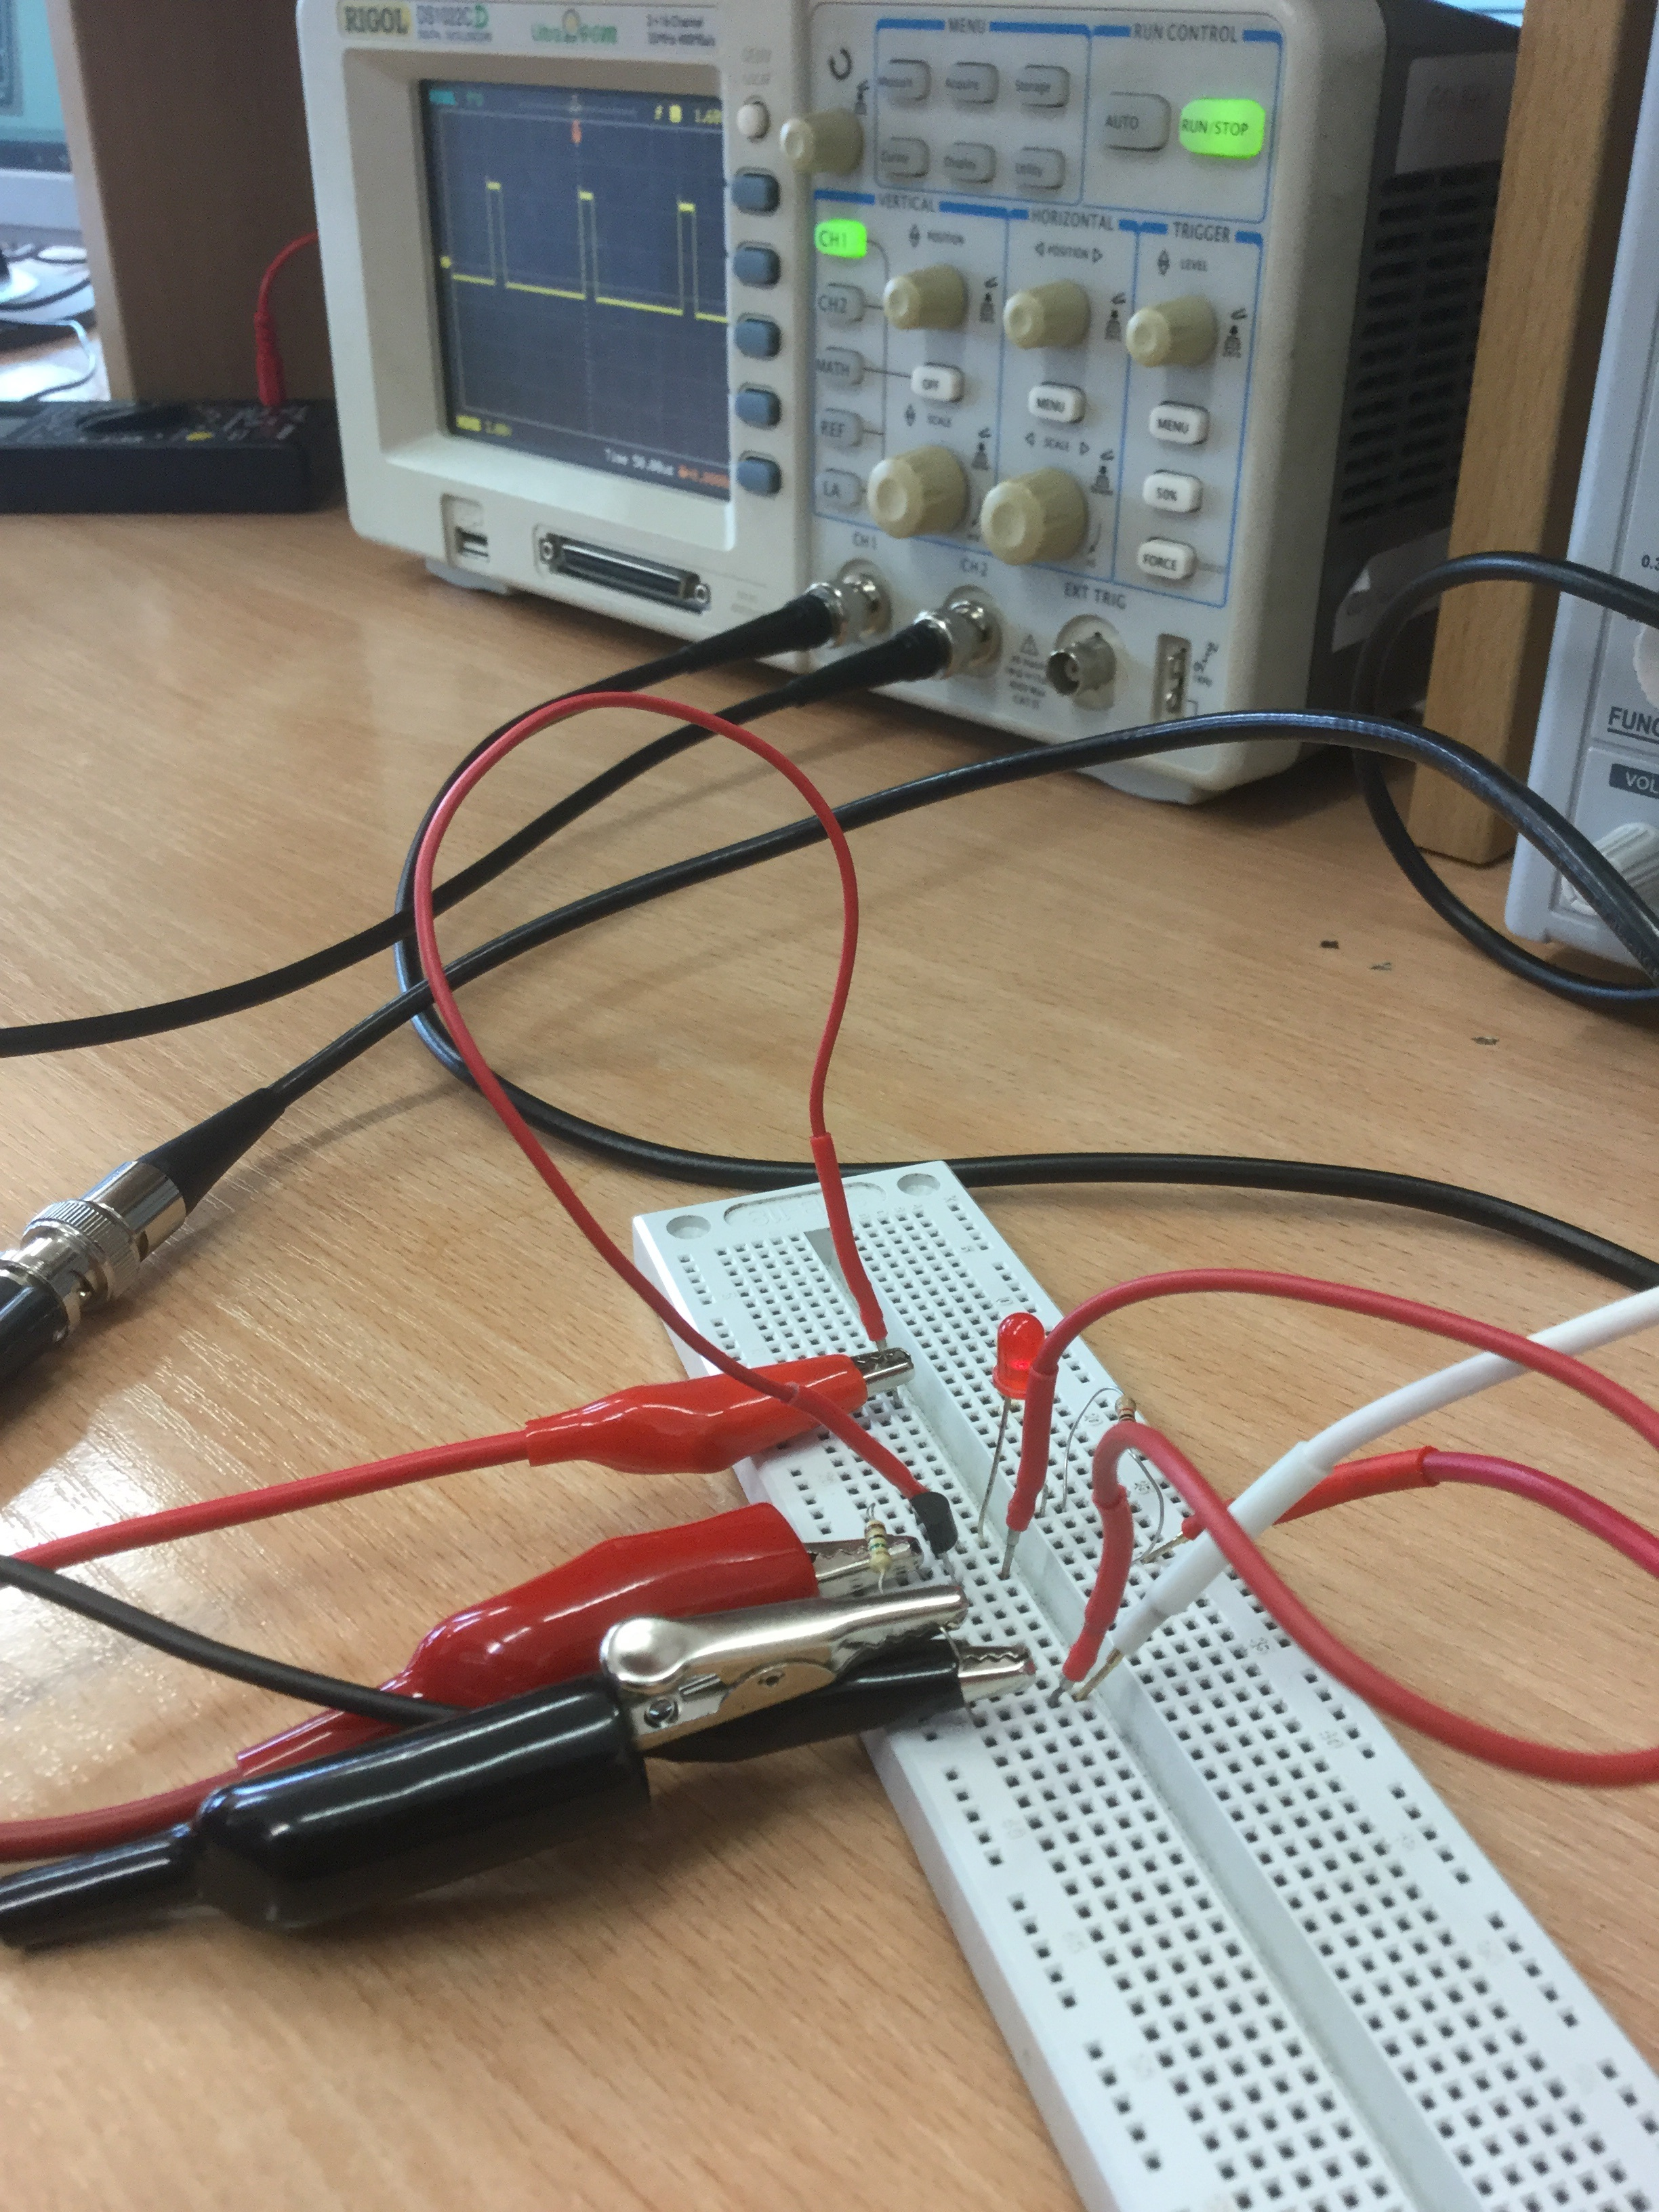
\includegraphics[scale=0.05]{male}
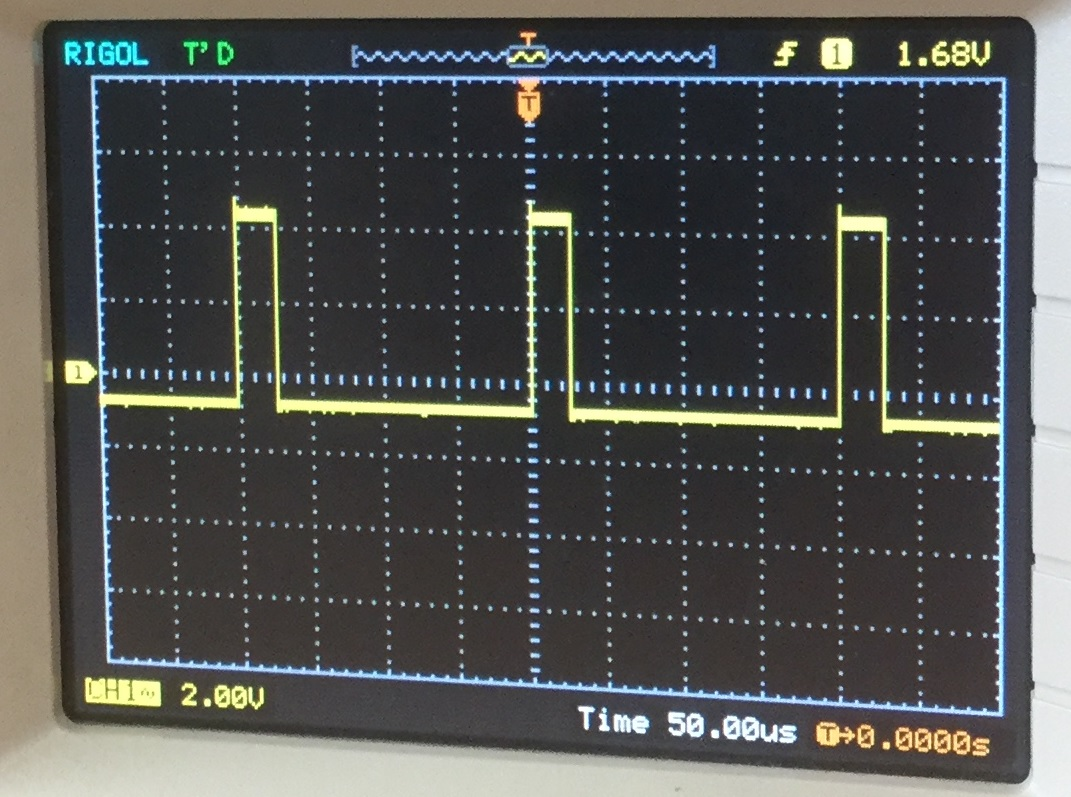
\includegraphics[scale=0.25]{maleOsc}

\caption{2) Duże wypełnienie}
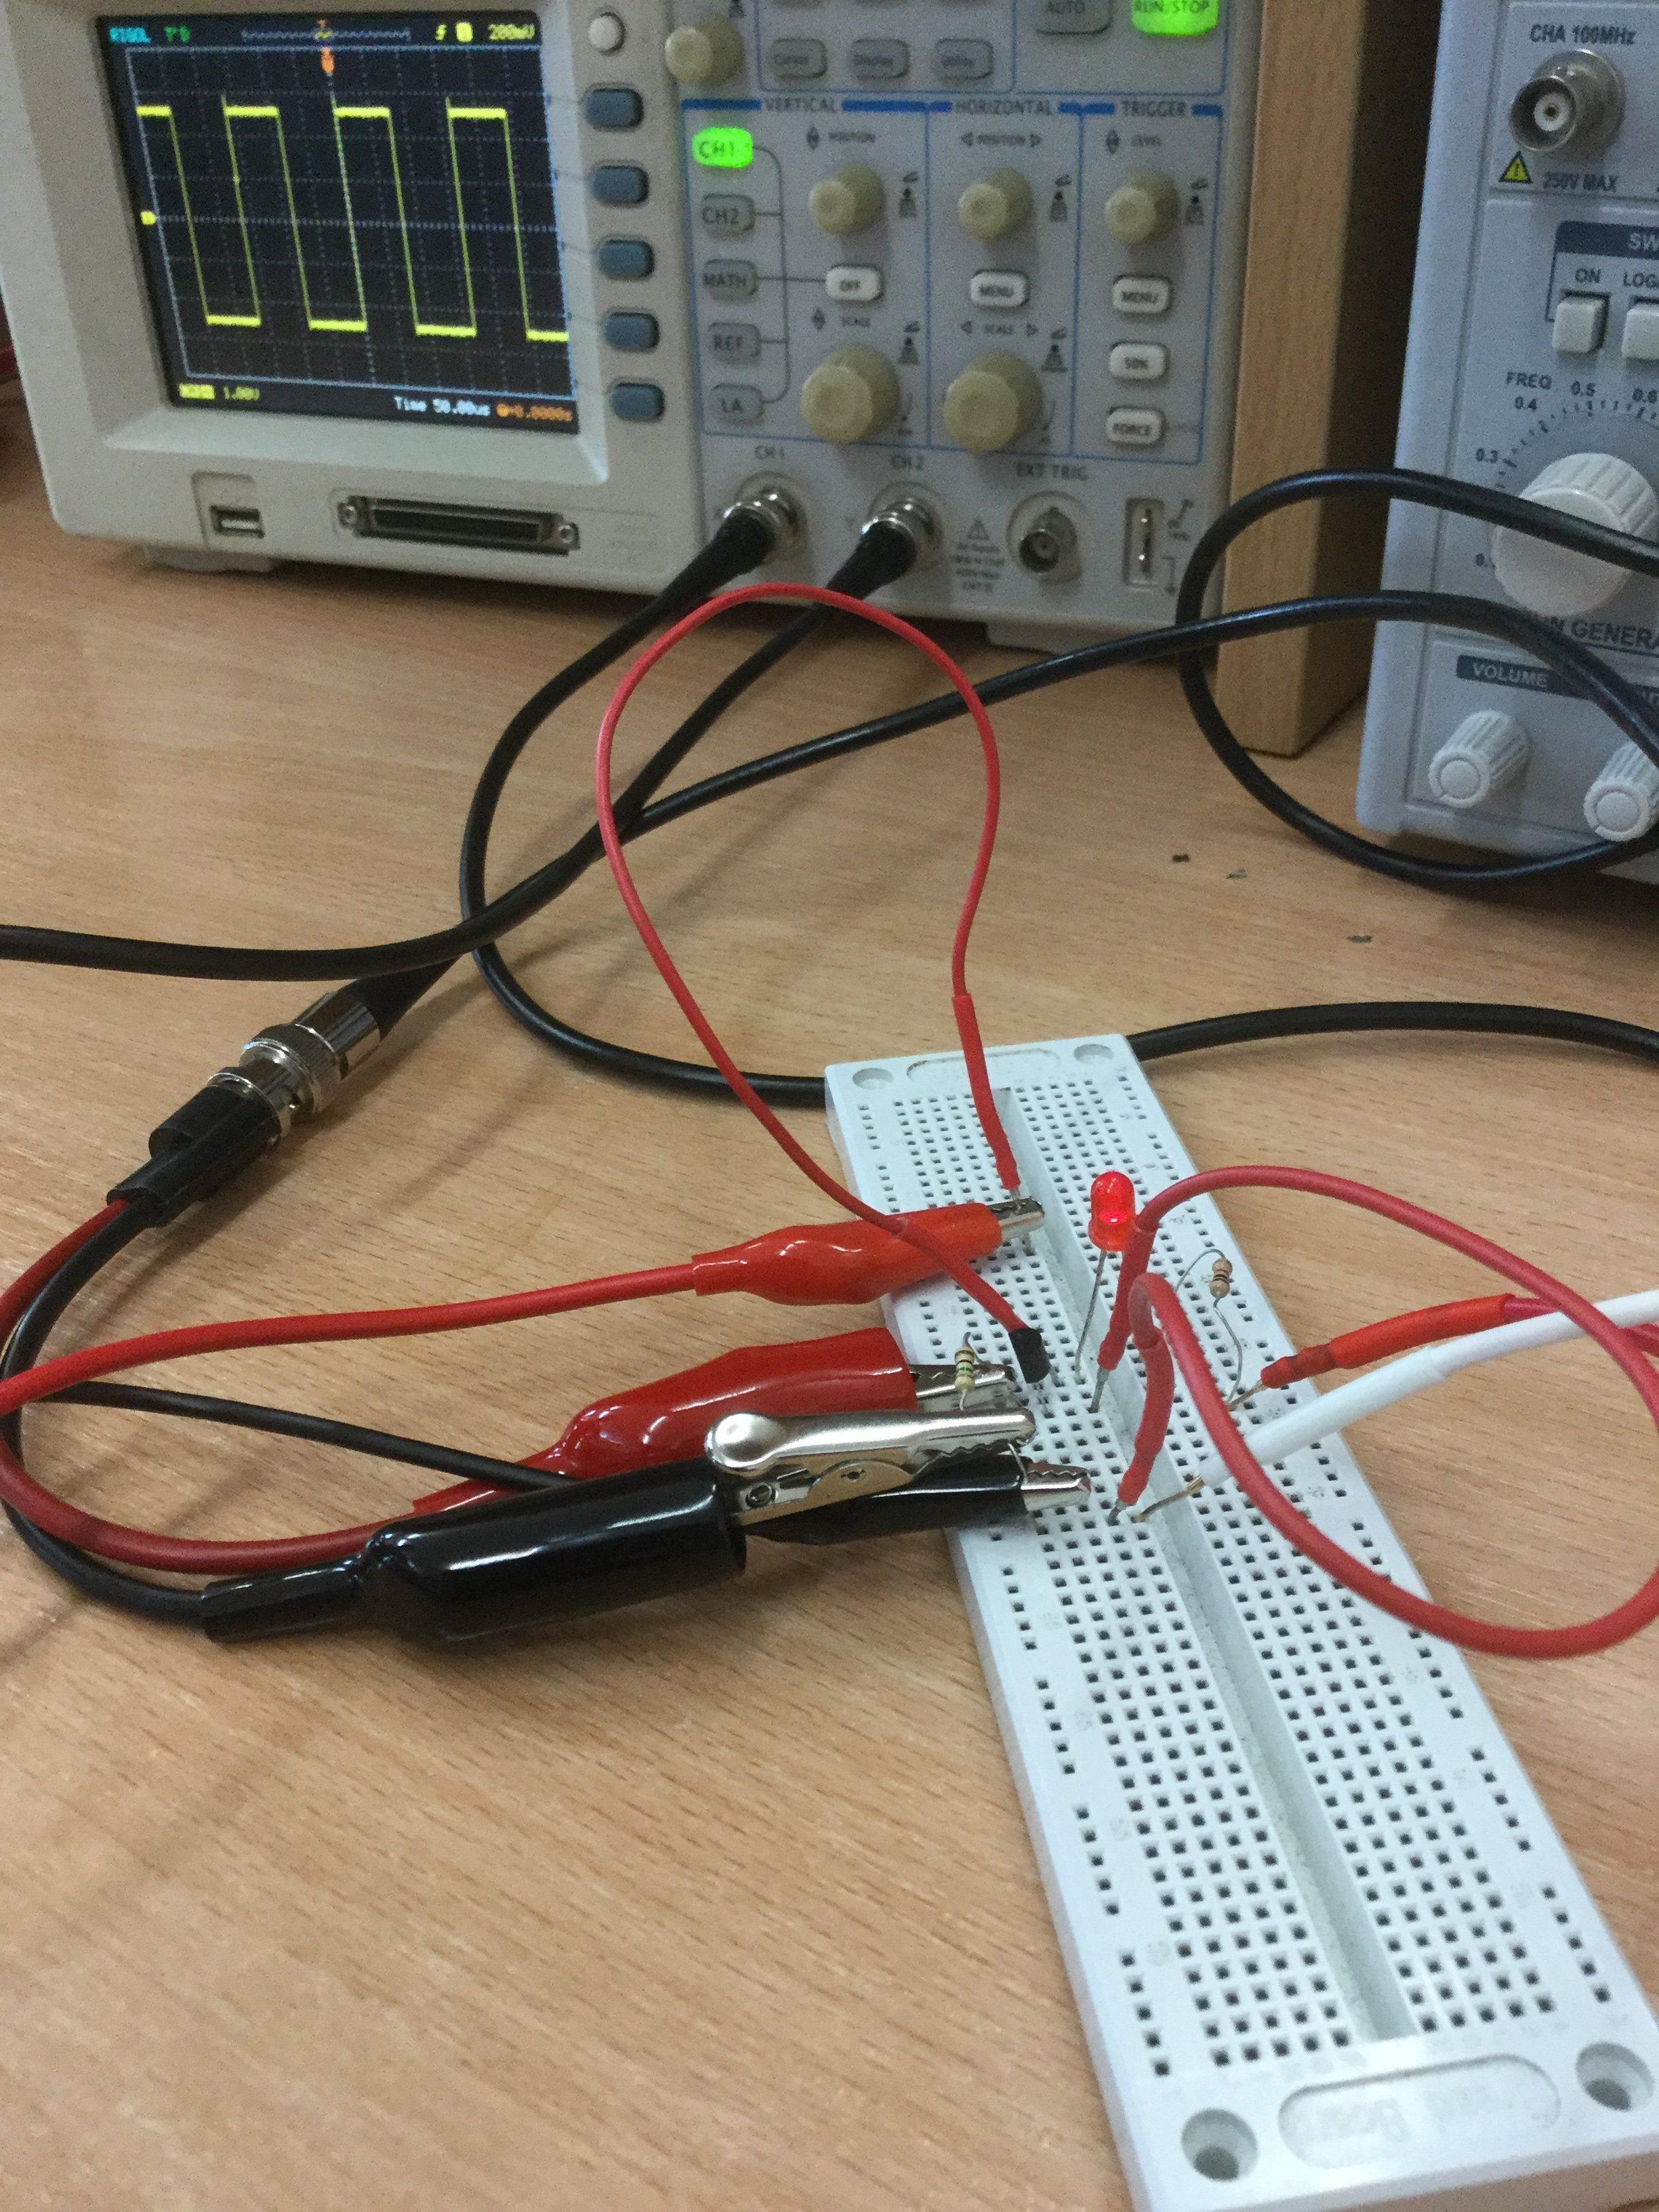
\includegraphics[scale=0.05]{duze}
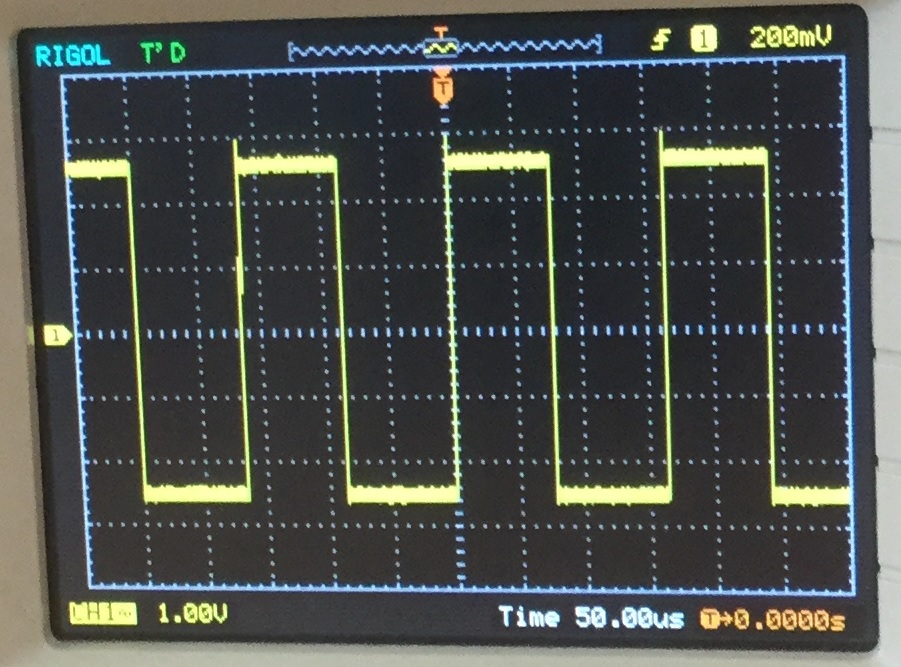
\includegraphics[scale=0.30]{duzeOsc}
\end{figure}

\newpage

\subsection*{5.}
Poniżej znajduje się oscylogram ukazujący przebieg sygnałów (w powiększeniu) dla częstotliwości pobudzenia $1,13Mhz$.\\
\begin{center}
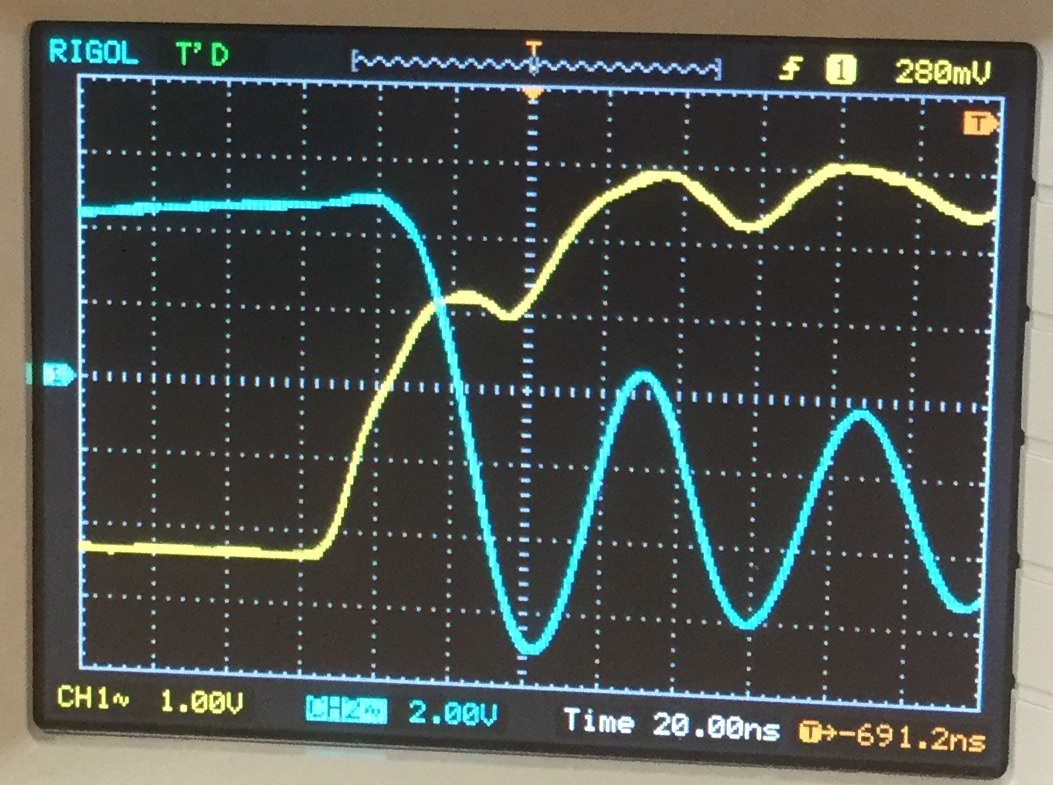
\includegraphics[scale=0.4]{oscylogram}
\end{center}

Z oscylogramu widać, że opóźnienie czasowe związane ze stanem przejściowym w pracy elementu to około $10ns$. 

\subsection*{6.}

Maksymalna częstotliwość stabilną pracy układu tranzystora i diody wyrażoną wzorem 
$$
f_{max} = \frac{1}{t_d}
$$
wynosi, dla $t_d = 10ns$, $f_{max} = 10^8 Hz = 100 MHz$.

\bibliography{IEEEabrv,refs}

\begin{thebibliography}{9}

\bibitem{rlc}
  W trakcie przeprowadzania doświadczeń i pisania sprawozdania zespół korzystał głównie z materiałów ze strony http://mariusznaumowicz.ddns.net/materialy.html oraz z wiedzy własnej.\\
Dane dotyczące tranzystorów pochodzą ze stron producentów: https://www.onsemi.com/pub/Collateral/BS170-D.PDF oraz http://www.vishay.com/docs/70209/70209.pdf.

\end{thebibliography}

\end{document}7